\documentclass[portrait,final,paperwidth=84.1cm,paperheight=118.9cm,fontscale=0.225,margin=50pt,american]{baposter}
% documentclass[]
\usepackage[T1]{fontenc}
\usepackage[latin9]{inputenc}
\usepackage{babel}
\usepackage{graphicx}
\usepackage{multicol}
\usepackage{scalefnt}
\usepackage{bm}
\usepackage{palatino}
\usepackage{url}
\usepackage{enumitem}
\usepackage{xcolor}
\usepackage{wasysym}

%%%%%%%%%%%%%%%%%%% Uni Tuebingen specific definitions %%%%%%%%%%%%%%%%%%%%
\input{environments.tex}
\renewcommand{\rmdefault}{phv} % Arial
\renewcommand{\sfdefault}{phv} % Arial
\newcommand{\todo}[1]{{\color{orange} #1}}

\setlength{\columnsep}{1.5em}
\setlength{\columnseprule}{0mm}

\newcommand{\compresslist}{%
  \setlength{\itemsep}{1pt}%
  \setlength{\parskip}{0pt}%
  \setlength{\parsep}{0pt}%
}

\setlength{\unitlength}{1mm}
\newcommand{\putpicture}[3]{\begin{picture}(0,0)\put(#1,#2){#3}\end{picture}}
\newcommand{\putgraphics}[4]{\begin{picture}(0,0)\put(#1,#2){\includegraphics[#3]{#4}}\end{picture}}








\begin{document}
%%%%%%%%%%%%%%%%%%%%%%%%%%%%%%%%%%%%%%%%%%%%%%%%%%%%%%%%%%%%%%%%%%%%%%%%%%%%%% 
%%% Here starts the poster
%%% ---------------------------------------------------------------------------
%%%%%%%%%%%%%%%%%%%%%%%%%%%%%%%%%%%%%%%%%%%%%%%%%%%%%%%%%%%%%%%%%%%%%%%%%%%%%% 


%%% Define UT colors
%%%%%%%%%%%%%%%%%%%%%%%%%%%%%%%%%%%%%%%%%%%%%%%%%%%%%%%%%%%%%%%%%%%%%%%%%%%%%% 

% Rand der Kästen
\definecolor{lightorange}{rgb}{0.9,0.4,0}
\definecolor{lightestorange}{rgb}{1,0.8,0.5}
% Überschriften Kästen
\definecolor{tured}{cmyk}{0, .8, .45, .27}


%%%%%%%%%%%%%%%%%%%%%%%%%%%%%%%%%%%%%%%%%%%%%%%%%%%%%%%%%%%%%%%%%%%%%%%%%%%%%% 
\begin{poster}
  % Poster Options
  {
    % Show grid to help with alignment
    grid=false,
    % Column spacing
    colspacing=1em,
    % Color style
    bgColorOne=white,
    bgColorTwo=white,
    %borderColor=sec03,
    borderColor=lightorange,
    %headerColorOne=sec02,
    headerColorOne=tured,
    headerColorTwo=sec21,
    headerFontColor=black,
    boxColorOne=white,
    boxColorTwo=white,
    % Format of textbox
    textborder=rectangle, %none,
    % Format of text header
    eyecatcher=true,
    columns=3,
    headerborder=closed,
    headerheight=0.19\textheight,
    footerheight=0.1\textheight,
    % textfont=\phv, %An example of changing the text font
    headershape=rectangle, %smallrounded,
    headershade=plain,
    headerfont=\bf\textsc, %Sans Serif
    % textfont={\setlength{\parindent}{1.5em}},
    boxshade=plain,
    % background=shade-tb,
    background=plain,
    linewidth=0.3ex
  }
  % Affiliation
   {
   Neuroethology Lab, Institute for Neurobiology, University of T\"ubingen
   }
  % Title
  {
  \vspace{-0mm}\putpicture{-80}{-23}{\includegraphics[height=8mm]{logo_all.pdf}}
  \scalefont{1}
  Random fish title with \textit{Apteronotus leptorhynchus}
  }
%short title} 
  % Authors
  {
    %\putpicture{-28}{0.5}{\includegraphics[height=1.75em]{./test.pdf}} 
    Jacqueline Laura G\"obl, Julia Gr\"ub, Max K\"uhn, Till Raab, Jan Benda\\[0.5ex]
    {\small till.raab@student.uni-tuebingen.de}
  }

%%%%%%%%%%%%%%%%%%%%%%%%%%%%%%%%%%%%%%%%%%%%%%%%%%%%%%%%%%%%%%%%%%%%%%%%%%%%%% 
%%% Now define the boxes that make up the poster
%%% ---------------------------------------------------------------------------
%%% Each box has a name and can be placed absolutely or relatively.
%%% The only inconvenience is that you can only specify a relative position 
%%% towards an already declared box. So if you have a box attached to the 
%%% bottom, one to the top and a third one which should be in between, you 
%%% have to specify the top and bottom boxes before you specify the middle 
%%% box.
%%%%%%%%%%%%%%%%%%%%%%%%%%%%%%%%%%%%%%%%%%%%%%%%%%%%%%%%%%%%%%%%%%%%%%%%%%%%%% 





%%%%%%%%%%%%%%%%%%%%%%%%%%%%%%%%%%%%%%%%%%%%%%%%%%%%%%%%%%%%%%%%%%%%%%%%%%%%%% 
\headerbox{Introduction}{name=intro, column=0, row=0}{
%%%%%%%%%%%%%%%%%%%%%%%%%%%%%%%%%%%%%%%%%%%%%%%%%%%%%%%%%%%%%%%%%%%%%%%%%%%%%% 

\scalefont{0.65}

Every species across the animal kingdom has its own way of life. While some species stay solitary for most of their life, others organize themselves in groups, where a hierarchical structure influences individual behaviors. Neotropical weakly electric fish continuously discharge an electric organ (EOD) and thereby generate a dipole like electric field used in navigation, foraging and communication. 
While the electrocommunication and -localization behaviors of these nocturnal animals are well studied, little is known about behaviors resulting from their social structure, especially over longer periods. To close this gap we track the spatio-temporal behavior of a group of \textit{A. leptorhynchus} housed in a large 2$^3$\,m indoor tank stocked with four natural-like habitats for ten consecutive days. The individually distinguishable electric field enable spatial tracking without the necessity of tagging and enable new insights into the dominance dependent spatio-temporal behaviors of the weakly electric fish \textit{A. leptorhynchus}.
}


%%%%%%%%%%%%%%%%%%%%%%%%%%%%%%%%%%%%%%%%%%%%%%%%%%%%%%%%%%%%%%%%%%%%%%%%%%%%%%
\headerbox{Conclusion}{name=conclusion, column=0, span = 2, above=bottom}{
%%%%%%%%%%%%%%%%%%%%%%%%%%%%%%%%%%%%%%%%%%%%%%%%%%%%%%%%%%%%%%%%%%%%%%%%%%%%%%

% \scalefont{0.65}
\scalefont{0.5}


\begin{itemize}
	\item 2 Spalten - eine pro research question?
	\item A) different species prefer different habitat characteristics
	\item A) wenn Platz, vielleicht nennen ?
	\item B) Zusammenhang Dominanz und habitat selection Apteronotus:
	\item B) dominantere Tiere eher in Steinen zu finden?
	\item B) ODER sinnvolles Fazit ziehen...
\end{itemize}
}



%%%%%%%%%%%%%%%%%%%%%%%%%%%%%%%%%%%%%%%%%%%%%%%%%%%%%%%%%%%%%%%%%%%%%%%%%%%%%% 
\headerbox{Results 1}{name=results1, column=0, span = 1, below=intro, above=conclusion}{
%%%%%%%%%%%%%%%%%%%%%%%%%%%%%%%%%%%%%%%%%%%%%%%%%%%%%%%%%%%%%%%%%%%%%%%%%%%%%% 

\scalefont{0.65}

%
% TITLE
\begin{center}
\vspace*{0.25cm}
\underline{Habitat Selection \& Water Flow}
\end{center}
%
% TEXT ABOVE
\begin{itemize}[leftmargin=0.43cm] \itemsep0pt
\item \textit{Apteronotus} preferres stones
\item \textit{Eigenmannia} preferes roots
\item Pulsefish prefer plants and roots
\end{itemize}
%
% PICTURE
\begin{center}
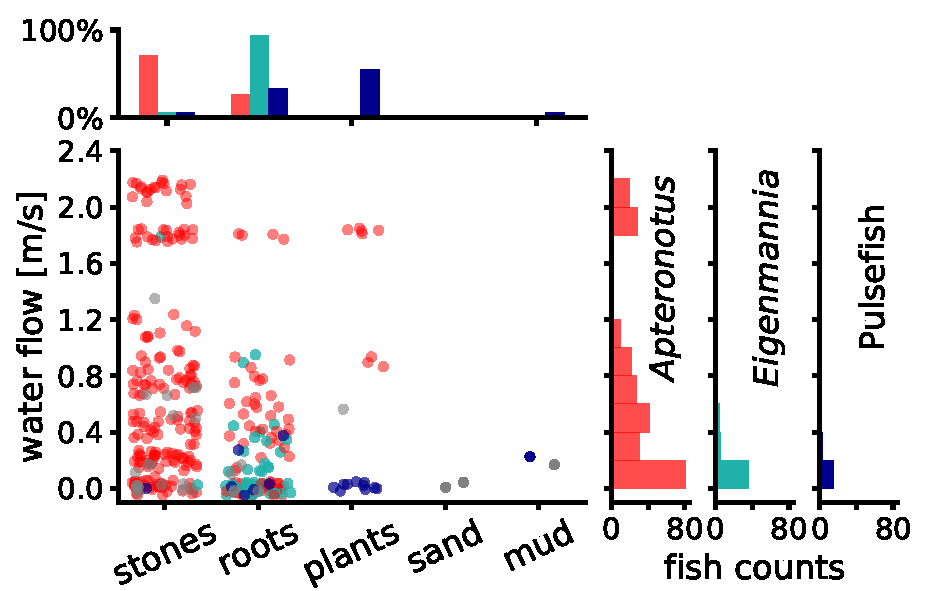
\includegraphics[width=\textwidth]{pictures/flow_habitat_poster.pdf}
\end{center}
%
% TEXT BELOW
\begin{itemize}[leftmargin=0.43cm] \itemsep0pt
\item \textit{Apteronotus} occurrs in wide range of water flow
\item \textit{Eigenmannia} prefers lower water speed (>~1~m/s)
\item Pulsefish prefer low water speed (>~0.4~m/s)
\end{itemize}
}

%%%%%%%%%%%%%%%%%%%%%%%%%%%%%%%%%%%%%%%%%%%%%%%%%%%%%%%%%%%%%%%%%%%%%%%%%%%%%% 
\headerbox{Results 2}{name=results2, column=1, span = 1, below=intro, above=conclusion}{
%%%%%%%%%%%%%%%%%%%%%%%%%%%%%%%%%%%%%%%%%%%%%%%%%%%%%%%%%%%%%%%%%%%%%%%%%%%%%% 

\scalefont{0.65}

%
% TITLE
\begin{center}
\vspace*{0.25cm}
\underline{Habitat Selection - Stones}
\end{center}
%
% PICTURE
\vspace*{-0.6cm}
\begin{center}
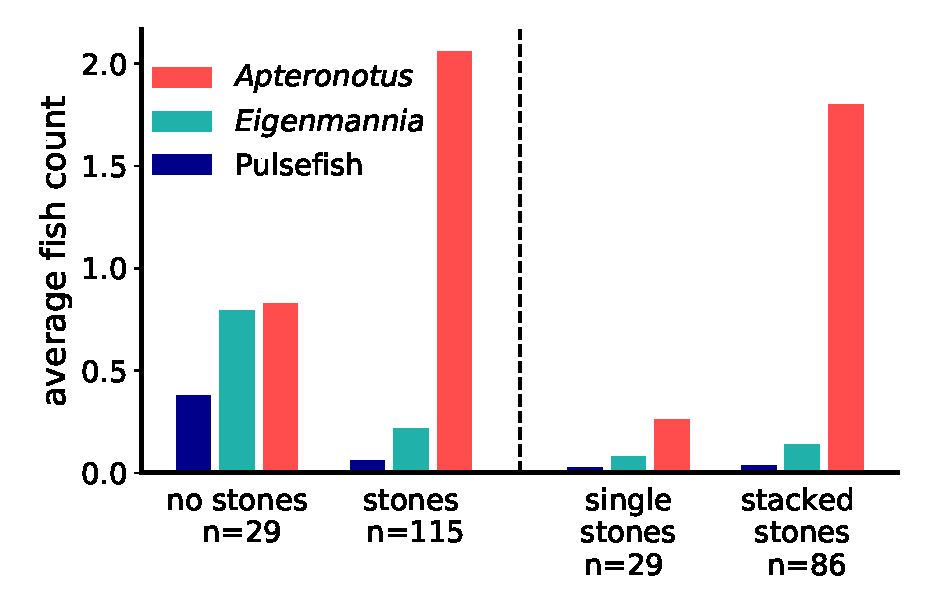
\includegraphics[width=\textwidth]{pictures/more_stones_pls_poster.pdf}
\end{center}
%
% TEXT BELOW
\begin{itemize}[leftmargin=0.43cm] \itemsep0pt
\item \textit{Apteronotus} clearly preferes stony habitats, or more precisely stacked stones
\item \textit{Eigenmannia} and Pulsefish show no preference towards stony habitats
\end{itemize}
}


%%%%%%%%%%%%%%%%%%%%%%%%%%%%%%%%%%%%%%%%%%%%%%%%%%%%%%%%%%%%%%%%%%%%%%%%%%%%%%
\headerbox{Results 3}{name=results3, column=2, span = 1, below=intro, above=bottom}{
%%%%%%%%%%%%%%%%%%%%%%%%%%%%%%%%%%%%%%%%%%%%%%%%%%%%%%%%%%%%%%%%%%%%%%%%%%%%%%

	\scalefont{0.65}
	%	
	% TITLE
	\begin{center}
	\underline{Habitat Selection \& Dominance in \textit{A. macrostomus}}
	\end{center}
	%
	% TEXT ABOVE
	\begin{itemize}[leftmargin=0.43cm] \itemsep0pt
	\item males and females differ in EODf
	\item in male \textit{Apteronoti}, a higher EODf is associated with dominance
	\item[-] \female: EODf $<$ 7xx~Hz
	\item[-] \mars: EODf $>$ 7xx~Hz
	\item[-] dominant \mars: EODf $>$ 8xx~Hz
	\end{itemize}
	%	
	% PICTURE
	\begin{center}
	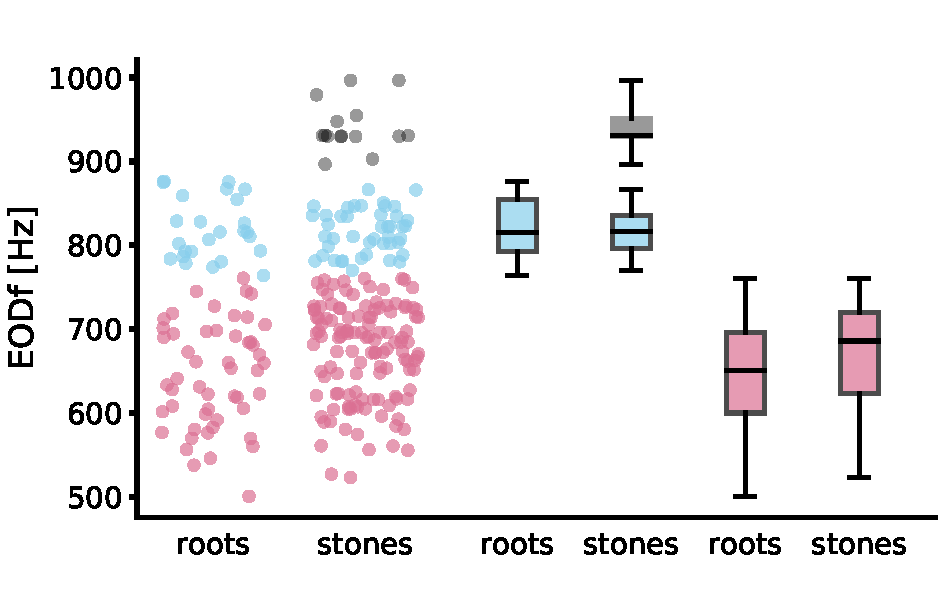
\includegraphics[width=\textwidth]{pictures/eod_habitat_poster.pdf}
	\end{center}
	% 
	% TEXT BELOW
	\begin{itemize}[leftmargin=0.43cm] \itemsep0pt
	\item females (pink) with higher EODf more often in stony habitats\\
	(TESTRESULTS)
	\item males with high dominance (grey) only in stony habitats\\
	(TESTRESULTS)
	\end{itemize}
}

%%%%%%%%%%%%%%%%%%%%%%%%%%%%%%%%%%%%%%%%%%%%%%%%%%%%%%%%%%%%%%%%%%%%%%%%%%%%%%
\headerbox{Methods}{name=methods, column=1, span=2, row=0, above=results1}{
%%%%%%%%%%%%%%%%%%%%%%%%%%%%%%%%%%%%%%%%%%%%%%%%%%%%%%%%%%%%%%%%%%%%%%%%%%%%%%
	
	\scalefont{0.65}
	
	%	
	% HEADER-LINES
	% ____________________________________________________________________	
	%	
	\fcolorbox{white}{white}{	
	\begin{minipage}[t]{.45\textwidth}
		\centering		
		\underline{Recording Site} % left
	\end{minipage}}
	\hspace{4ex}
	\fcolorbox{white}{white}{	
	\begin{minipage}[t]{.45\textwidth}
		\centering		
		\underline{Species Discrimination} % right
	\end{minipage}}
	%	
	% LEFT AREA
	% ____________________________________________________________________	
	%
	\fcolorbox{white}{white}{		
	\begin{minipage}[b][7.1cm][t]{.45\textwidth}
		%		
		% PICTURE 		
		\begin{center}
		\includegraphics[width=\textwidth]{pictures/POSTER_habitats.pdf} 
		\end{center}
		%
		% TEXT BELOW
		\vspace*{-0.5cm}
		\begin{itemize}[leftmargin=0.3cm] \itemsep0pt
		\item daytime field recordings, October 2020
		\item Rio Canomamao, Reserva el Caduceo, San Martin, Meta, Colombia
		\end{itemize}				
	\end{minipage}}
	\hspace{4ex}
	%
	% RIGHT AREA
	% _____________________________________________________________________
	%
	\fcolorbox{white}{white}{		
	\begin{minipage}[b][7.1cm][t]{.45\textwidth}
		%
		% PICTURE		
		\begin{center}
		\includegraphics[width=\textwidth]{pictures/count_ampl_EODf_waveforms_bearbeitet.pdf} 
		\end{center}
		%
		% TEXT BELOW
		\vspace*{-0.5cm}
		\begin{itemize}[leftmargin=0.43cm] \itemsep0pt
		\item separation between pulse- and wave-type species via Thunderfish TM
		\item Differentiation between different wave-type species due to species-specific EODf and waveform characteristics (relative peak to peak amplitude, RPA)
		\end{itemize}
	\end{minipage}}
}

\end{poster}
\end{document}

